% Options for packages loaded elsewhere
\PassOptionsToPackage{unicode}{hyperref}
\PassOptionsToPackage{hyphens}{url}
%
\documentclass[
]{article}
\usepackage{amsmath,amssymb}
\usepackage{lmodern}
\usepackage{iftex}
\ifPDFTeX
  \usepackage[T1]{fontenc}
  \usepackage[utf8]{inputenc}
  \usepackage{textcomp} % provide euro and other symbols
\else % if luatex or xetex
  \usepackage{unicode-math}
  \defaultfontfeatures{Scale=MatchLowercase}
  \defaultfontfeatures[\rmfamily]{Ligatures=TeX,Scale=1}
\fi
% Use upquote if available, for straight quotes in verbatim environments
\IfFileExists{upquote.sty}{\usepackage{upquote}}{}
\IfFileExists{microtype.sty}{% use microtype if available
  \usepackage[]{microtype}
  \UseMicrotypeSet[protrusion]{basicmath} % disable protrusion for tt fonts
}{}
\makeatletter
\@ifundefined{KOMAClassName}{% if non-KOMA class
  \IfFileExists{parskip.sty}{%
    \usepackage{parskip}
  }{% else
    \setlength{\parindent}{0pt}
    \setlength{\parskip}{6pt plus 2pt minus 1pt}}
}{% if KOMA class
  \KOMAoptions{parskip=half}}
\makeatother
\usepackage{xcolor}
\usepackage[margin=1in]{geometry}
\usepackage{color}
\usepackage{fancyvrb}
\newcommand{\VerbBar}{|}
\newcommand{\VERB}{\Verb[commandchars=\\\{\}]}
\DefineVerbatimEnvironment{Highlighting}{Verbatim}{commandchars=\\\{\}}
% Add ',fontsize=\small' for more characters per line
\newenvironment{Shaded}{}{}
\newcommand{\AlertTok}[1]{\textcolor[rgb]{1.00,0.00,0.00}{\textbf{#1}}}
\newcommand{\AnnotationTok}[1]{\textcolor[rgb]{0.38,0.63,0.69}{\textbf{\textit{#1}}}}
\newcommand{\AttributeTok}[1]{\textcolor[rgb]{0.49,0.56,0.16}{#1}}
\newcommand{\BaseNTok}[1]{\textcolor[rgb]{0.25,0.63,0.44}{#1}}
\newcommand{\BuiltInTok}[1]{#1}
\newcommand{\CharTok}[1]{\textcolor[rgb]{0.25,0.44,0.63}{#1}}
\newcommand{\CommentTok}[1]{\textcolor[rgb]{0.38,0.63,0.69}{\textit{#1}}}
\newcommand{\CommentVarTok}[1]{\textcolor[rgb]{0.38,0.63,0.69}{\textbf{\textit{#1}}}}
\newcommand{\ConstantTok}[1]{\textcolor[rgb]{0.53,0.00,0.00}{#1}}
\newcommand{\ControlFlowTok}[1]{\textcolor[rgb]{0.00,0.44,0.13}{\textbf{#1}}}
\newcommand{\DataTypeTok}[1]{\textcolor[rgb]{0.56,0.13,0.00}{#1}}
\newcommand{\DecValTok}[1]{\textcolor[rgb]{0.25,0.63,0.44}{#1}}
\newcommand{\DocumentationTok}[1]{\textcolor[rgb]{0.73,0.13,0.13}{\textit{#1}}}
\newcommand{\ErrorTok}[1]{\textcolor[rgb]{1.00,0.00,0.00}{\textbf{#1}}}
\newcommand{\ExtensionTok}[1]{#1}
\newcommand{\FloatTok}[1]{\textcolor[rgb]{0.25,0.63,0.44}{#1}}
\newcommand{\FunctionTok}[1]{\textcolor[rgb]{0.02,0.16,0.49}{#1}}
\newcommand{\ImportTok}[1]{#1}
\newcommand{\InformationTok}[1]{\textcolor[rgb]{0.38,0.63,0.69}{\textbf{\textit{#1}}}}
\newcommand{\KeywordTok}[1]{\textcolor[rgb]{0.00,0.44,0.13}{\textbf{#1}}}
\newcommand{\NormalTok}[1]{#1}
\newcommand{\OperatorTok}[1]{\textcolor[rgb]{0.40,0.40,0.40}{#1}}
\newcommand{\OtherTok}[1]{\textcolor[rgb]{0.00,0.44,0.13}{#1}}
\newcommand{\PreprocessorTok}[1]{\textcolor[rgb]{0.74,0.48,0.00}{#1}}
\newcommand{\RegionMarkerTok}[1]{#1}
\newcommand{\SpecialCharTok}[1]{\textcolor[rgb]{0.25,0.44,0.63}{#1}}
\newcommand{\SpecialStringTok}[1]{\textcolor[rgb]{0.73,0.40,0.53}{#1}}
\newcommand{\StringTok}[1]{\textcolor[rgb]{0.25,0.44,0.63}{#1}}
\newcommand{\VariableTok}[1]{\textcolor[rgb]{0.10,0.09,0.49}{#1}}
\newcommand{\VerbatimStringTok}[1]{\textcolor[rgb]{0.25,0.44,0.63}{#1}}
\newcommand{\WarningTok}[1]{\textcolor[rgb]{0.38,0.63,0.69}{\textbf{\textit{#1}}}}
\usepackage{graphicx}
\makeatletter
\def\maxwidth{\ifdim\Gin@nat@width>\linewidth\linewidth\else\Gin@nat@width\fi}
\def\maxheight{\ifdim\Gin@nat@height>\textheight\textheight\else\Gin@nat@height\fi}
\makeatother
% Scale images if necessary, so that they will not overflow the page
% margins by default, and it is still possible to overwrite the defaults
% using explicit options in \includegraphics[width, height, ...]{}
\setkeys{Gin}{width=\maxwidth,height=\maxheight,keepaspectratio}
% Set default figure placement to htbp
\makeatletter
\def\fps@figure{htbp}
\makeatother
\setlength{\emergencystretch}{3em} % prevent overfull lines
\providecommand{\tightlist}{%
  \setlength{\itemsep}{0pt}\setlength{\parskip}{0pt}}
\setcounter{secnumdepth}{5}
\ifLuaTeX
  \usepackage{selnolig}  % disable illegal ligatures
\fi
\IfFileExists{bookmark.sty}{\usepackage{bookmark}}{\usepackage{hyperref}}
\IfFileExists{xurl.sty}{\usepackage{xurl}}{} % add URL line breaks if available
\urlstyle{same} % disable monospaced font for URLs
\hypersetup{
  pdftitle={Cómo instalar R y Rstudio y generar un proyecto},
  hidelinks,
  pdfcreator={LaTeX via pandoc}}

\title{Cómo instalar R y Rstudio y generar un proyecto}
\usepackage{etoolbox}
\makeatletter
\providecommand{\subtitle}[1]{% add subtitle to \maketitle
  \apptocmd{\@title}{\par {\large #1 \par}}{}{}
}
\makeatother
\subtitle{Curso: Estadística Aplicada y Procesamiento de Datos con R}
\author{}
\date{\vspace{-2.5em}August 16, 2022}

\begin{document}
\maketitle

{
\setcounter{tocdepth}{4}
\tableofcontents
}
\begin{Shaded}
\begin{Highlighting}[]
\CommentTok{\# output:}

\FunctionTok{rm}\NormalTok{(}\AttributeTok{list=}\FunctionTok{ls}\NormalTok{());}\FunctionTok{gc}\NormalTok{() }\CommentTok{\#Siempre es necesario borrar la memoria de 0 antes de correr un proyecto. }
\end{Highlighting}
\end{Shaded}

\begin{verbatim}
##          used (Mb) gc trigger (Mb) max used (Mb)
## Ncells 479765 25.7    1051432 56.2   638648 34.2
## Vcells 841093  6.5    8388608 64.0  1632242 12.5
\end{verbatim}

\begin{Shaded}
\begin{Highlighting}[]
\CommentTok{\#Lo anterior para chequear que no hayan objetos (información como bases de datos, }
\CommentTok{\#nombres de columnas, etiquetas, etc.) anidados que no estamos llamando, }
\FunctionTok{unlink}\NormalTok{(}\StringTok{\textquotesingle{}*\_cache\textquotesingle{}}\NormalTok{, }\AttributeTok{recursive =} \ConstantTok{TRUE}\NormalTok{) }\CommentTok{\#También limpiamos la memoria caché de cualquier otro elemento }
\CommentTok{\#que esté alojado en nuestra memoria. Recuerde que quien abra su proyecto no }
\CommentTok{\#contará con otro objeto que los que llame conforme a las instrucciones que escriba en el documento.}

\CommentTok{\#Veo desde donde consigo los datos, desde que servidor de R}
\CommentTok{\# Esta es una de las direcciones del CRAN (Comprehensive R Archive Network) correspondiente a Chile. }
\CommentTok{\#Es recomendable definir por defecto un CRAN cercano. }
\FunctionTok{options}\NormalTok{(}\AttributeTok{repos=}\FunctionTok{structure}\NormalTok{(}\FunctionTok{c}\NormalTok{(}\AttributeTok{CRAN=}\StringTok{"https://cran.dcc.uchile.cl/"}\NormalTok{))) }

\NormalTok{knitr}\SpecialCharTok{::}\NormalTok{opts\_chunk}\SpecialCharTok{$}\FunctionTok{set}\NormalTok{(}\AttributeTok{echo =} \ConstantTok{TRUE}\NormalTok{)}

\CommentTok{\#instalo lo que instala paquetes}
\ControlFlowTok{if}\NormalTok{(}\SpecialCharTok{!}\FunctionTok{require}\NormalTok{(pacman))\{}\FunctionTok{install.packages}\NormalTok{(}\StringTok{"pacman"}\NormalTok{)\}}
\end{Highlighting}
\end{Shaded}

\begin{verbatim}
## Loading required package: pacman
\end{verbatim}

\begin{verbatim}
## Warning: package 'pacman' was built under R version 4.0.3
\end{verbatim}

\begin{Shaded}
\begin{Highlighting}[]
\CommentTok{\#INSTALO PAQUETES}
\NormalTok{pacman}\SpecialCharTok{::}\FunctionTok{p\_load}\NormalTok{(knitr, dplyr)}
\ControlFlowTok{if}\NormalTok{(}\SpecialCharTok{!}\FunctionTok{require}\NormalTok{(tiktokrmd))\{remotes}\SpecialCharTok{::}\FunctionTok{install\_github}\NormalTok{(}\StringTok{"gadenbuie/tiktokrmd@main"}\NormalTok{)\}}
\end{Highlighting}
\end{Shaded}

\begin{verbatim}
## Loading required package: tiktokrmd
\end{verbatim}

\hypertarget{cuxf3mo-bajar-r-y-rstudio}{%
\section{Cómo bajar R y Rstudio}\label{cuxf3mo-bajar-r-y-rstudio}}

Este tutorial sólo es \textbf{uno de muchos que usted podrá encontrar
para instalar estos programas}. Posiblemente, existan alternativas mucho
más personalizadas para instalar R y Rstudio en línea. Ahora bien, creo
firmemente en que esta es la opción más \textbf{rápida y simple} de
instalarlos, por lo que recomiendo que en una primera instancia
\textbf{no se aleje de las instrucciones}, de lo contrario tendrá
problemas para instalar el programa y no podrá avanzar en las etapas del
taller.

\hypertarget{paso-1-bajar-r}{%
\subsection{Paso 1: Bajar R}\label{paso-1-bajar-r}}

Haga click en el siguiente enlace si usted tiene de sistema operativo
Windows \url{https://cran.r-project.org/bin/windows/base/}. Posiblemente
y si se lo solicita el programa, una vez que instale R y Rstudio deberá
instalar Rtools (\url{https://cran.r-project.org/bin/windows/Rtools/}).
\textbf{Pueda dar doble click para acercar la imagen si abre este
archivo en .html}

\begin{center}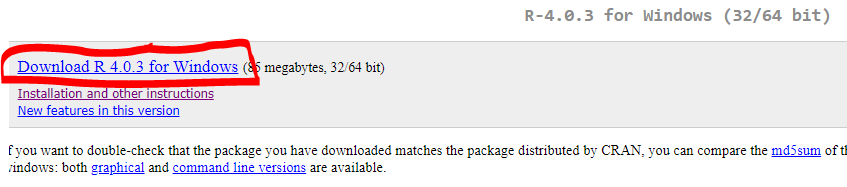
\includegraphics[width=11.76in]{./figs/Instalacion R- Win (0)} \end{center}

Si usted tiene un MAC, favor dirigirse a este enlace:
\url{https://cran.r-project.org/bin/macosx/}.

\begin{center}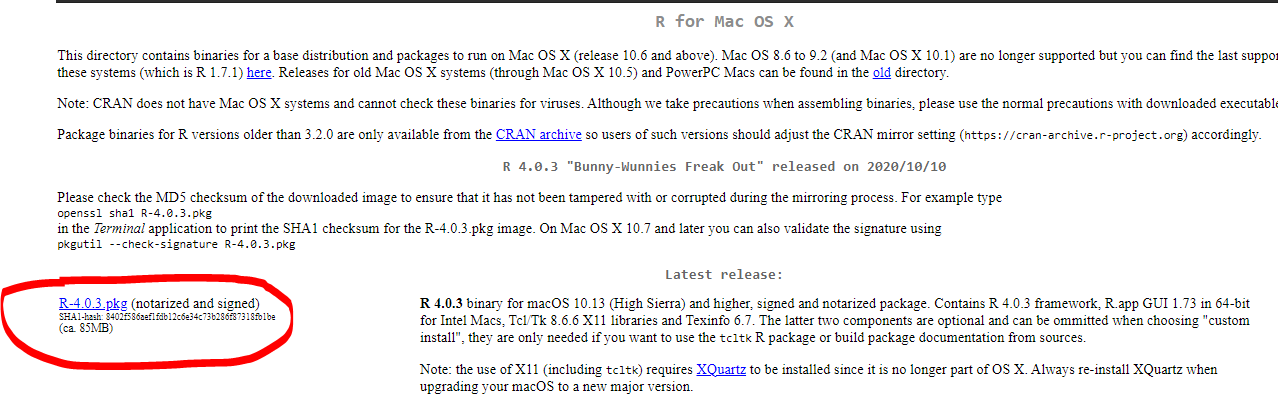
\includegraphics[width=17.75in]{./figs/Instalacion R- MAC (0)} \end{center}

O por último, puede encontrar aquí una alternativa plausible para MacOS
para bajar R y Rstudio:

\textbf{Advertencia:} Favor siga las instrucciones al momento de bajar
los archivos. Es necesario que instale en primer lugar R commander, y
posteriormente RStudio. Si usted ya bajó una versión de R o RStudio que
no ha funcionado bien, que cree muy desactualizada o que nunca supo
ocupar, \textbf{favor desinstalarlo(s) y reiniciar su computador}.

\hypertarget{paso-2-instalar-r-ejemplo-en-windows}{%
\subsection{Paso 2: Instalar R (ejemplo en
Windows)}\label{paso-2-instalar-r-ejemplo-en-windows}}

A continuación, pueden ver las capturas de pantalla de una instalación
en windows. Favor seguir todos los pasos.

\begin{center}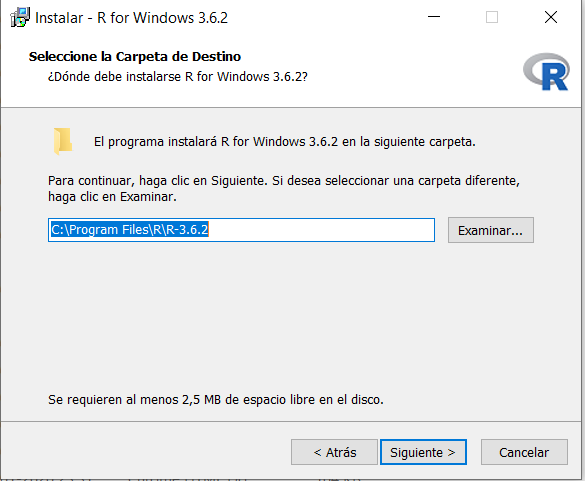
\includegraphics[width=8.12in]{./figs/Instalacion R- Win (2)} \end{center}

\begin{center}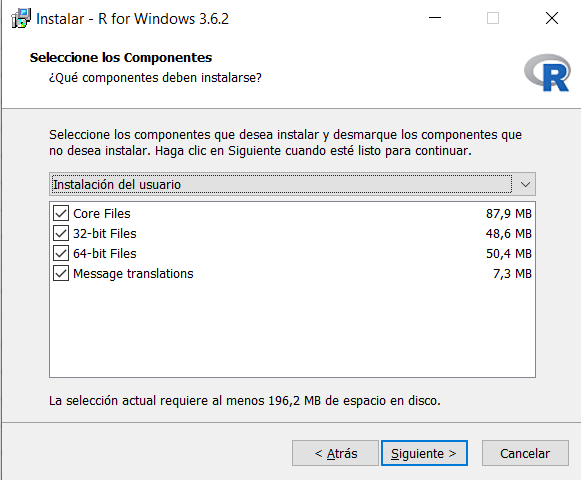
\includegraphics[width=8.07in]{./figs/Instalacion R- Win (3)} \end{center}

\begin{center}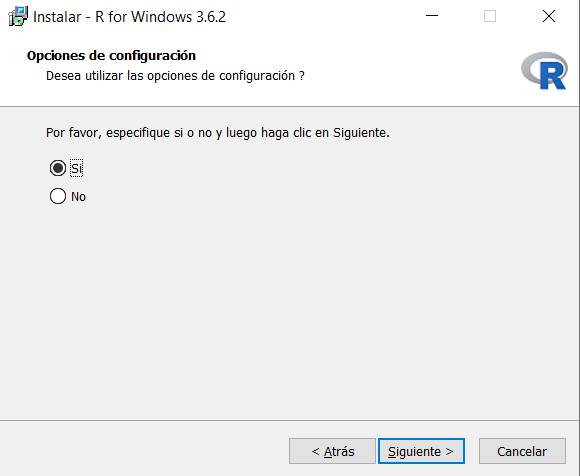
\includegraphics[width=8.06in]{./figs/Instalacion R- Win (4)} \end{center}

\begin{center}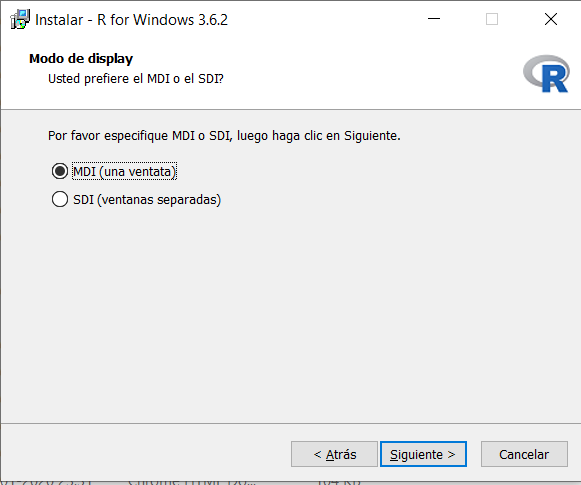
\includegraphics[width=8.07in]{./figs/Instalacion R- Win (5)} \end{center}

\begin{center}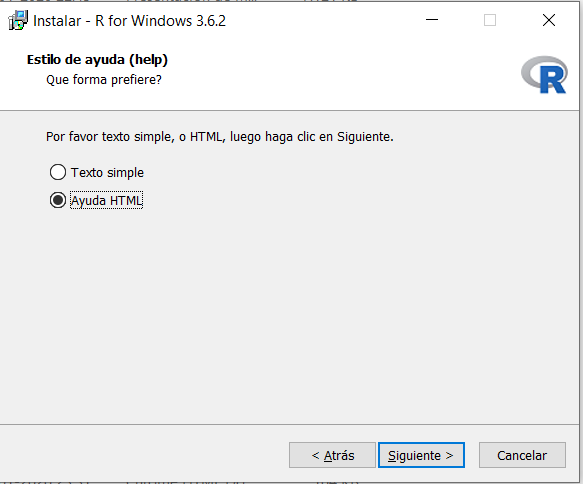
\includegraphics[width=8.1in]{./figs/Instalacion R- Win (6)} \end{center}

\begin{center}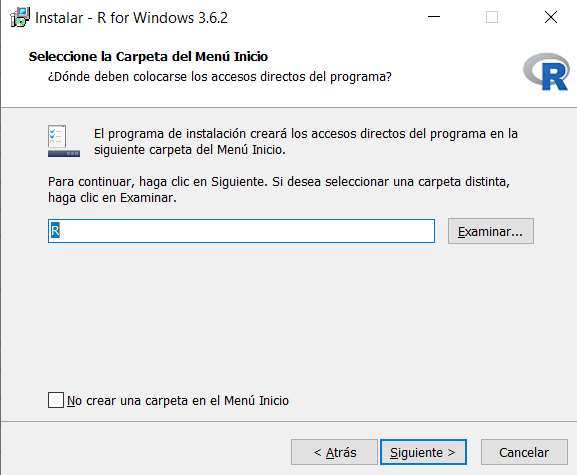
\includegraphics[width=8.01in]{./figs/Instalacion R- Win (7)} \end{center}

\textbf{Observación:} Favor no abrir R directamente, sino sólo a través
de R Studio. Dejar vacío los cuadros contorneados por la línea roja.

\begin{center}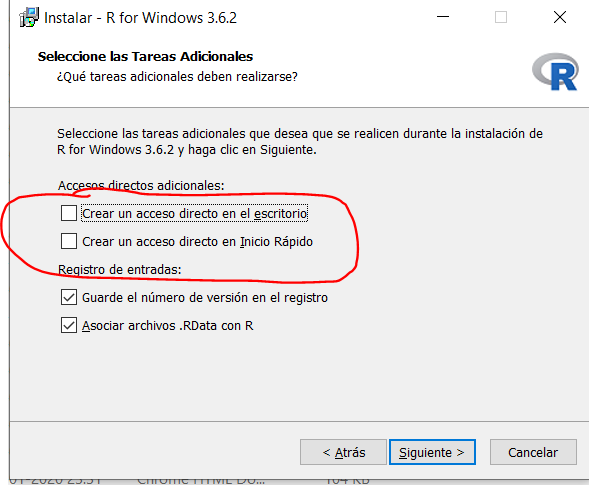
\includegraphics[width=0.6\linewidth]{./figs/Instalacion R- Win (8)} \end{center}

\hypertarget{paso-3-bajar-e-instalar-rstudio}{%
\subsection{Paso 3: Bajar e instalar
RStudio}\label{paso-3-bajar-e-instalar-rstudio}}

Una vez \textbf{reiniciado el computador} y habiendo cumplido con el
paso previo, diríjase al siguiente enlace
(\url{https://rstudio.com/products/rstudio/download/\#download}).
Seleccione el instalador que se adapte a la capacidad de su computador.
Debe tener en cuenta que si su computador no se encuentra actualizado a
sistemas operativos más recientes, no podrá contar con la última versión
de los productos presetados aquí.

\begin{center}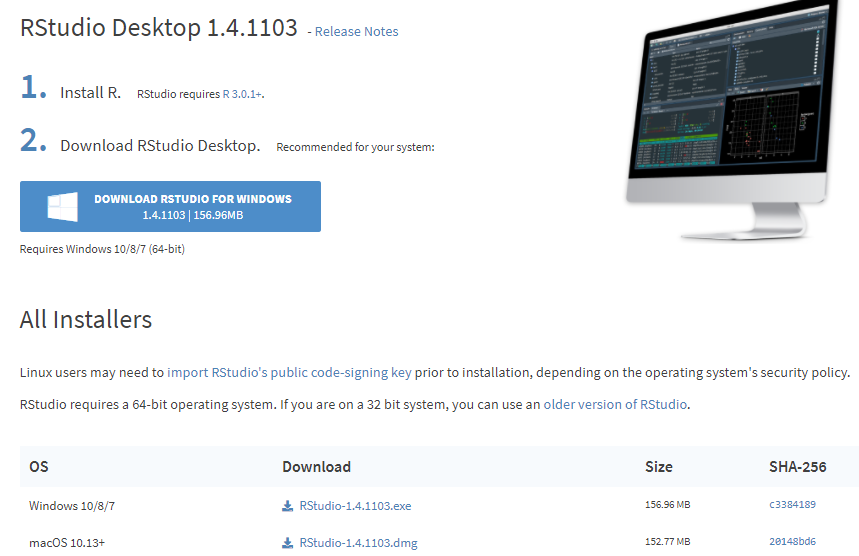
\includegraphics[width=0.6\linewidth]{./figs/Instalacion R- Win (9)} \end{center}

A continuación se muestra cómo bajarlo para Windows:

\begin{center}\includegraphics{./figs/instalacion_Rstudio1} \end{center}

Una vez ya bajado de internet, favor abrir y apretar el botón siguiente
en todos sus campos. \textbf{Observación}: Existen opciones para
personalizar las acciones que hicimos aquí. De todas formas este es un
taller introductorio, por lo que no se ahondarán en estas alternativas.

\begin{center}\includegraphics{./figs/instalacion_Rstudio2} \end{center}

\textbf{Reinicie el computador una vez finalizada la instalación}

\hypertarget{paso-4-prueba-opcional}{%
\subsection{Paso 4: Prueba (Opcional)}\label{paso-4-prueba-opcional}}

Abra una nueva sesión en Rstudio (abra el programa).

Habiendo cumplido con el paso previo, abra R Studio y corra el siguiente
comando en la Consola (siga los pasos de la imagen):
\texttt{install.packages("janitor")}.

\begin{center}\includegraphics{./figs/instalacion_Rstudio3} \end{center}

¿Obtuvo el siguiente mensaje?, si lo obtuvo es porque la instalación fue
exitosa.

\begin{center}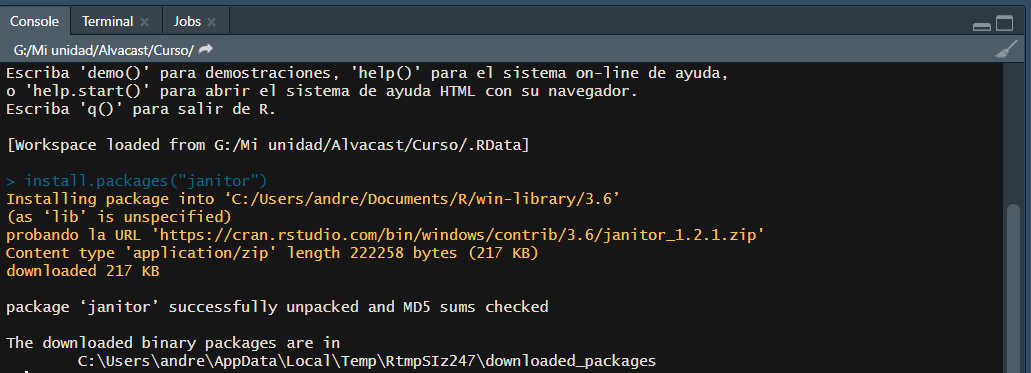
\includegraphics[width=14.32in]{./figs/Instalacion_final} \end{center}

\hypertarget{comentarios-y-dificultades-del-proceso-de-instalaciuxf3n}{%
\subsection{Comentarios y Dificultades del Proceso de
Instalación}\label{comentarios-y-dificultades-del-proceso-de-instalaciuxf3n}}

Si presenta problemas, favor dirigirse al siguiente enlace y reportarlo:
{
\href{https://docs.google.com/forms/d/e/1FAIpQLSdPhIwiY_7at09GM-KkAgklmWHamWcWaPY-yeoPVMoWeIRI2w/viewform?usp=sf_link}{\textbf{ENLACE}}
}

Si requiere instalar en Ubuntu, favor ver el siguiente enlace:
\url{https://www.digitalocean.com/community/tutorials/how-to-install-r-on-ubuntu-20-04}

\begin{center}\rule{0.5\linewidth}{0.5pt}\end{center}

\hypertarget{cuxf3mo-hacer-un-proyecto}{%
\section{¿Cómo hacer un proyecto?}\label{cuxf3mo-hacer-un-proyecto}}

\begin{itemize}
\tightlist
\item
  RStudio tiene la gran ventaja de que permite diferenciar proyectos en
  que el entorno será distinto
\end{itemize}

\textbf{ES MUY IMPORTANTE QUE DEFINAN UNA CARPETA PARA CADA UNO DE SUS
PROYECTOS. ES UNA MUY BUENA PRÁCTICA. PORQUE ASÍ LES VA A LEER DE MANERA
MÁS FÁCIL LOS ARCHIVOS COMO IMAGENES QUE QUIERAN CARGAR, BASES DE DATOS,
ETC.}

\hypertarget{paso-1.-nuevo-proyecto}{%
\subsection{Paso 1. Nuevo proyecto}\label{paso-1.-nuevo-proyecto}}

\begin{itemize}
\tightlist
\item
  Abro Rstudio, voy a la carpeta y abro New Project (\textbf{haga click
  en las imágenes para ampliarlas, si lo abren en .html}).
\end{itemize}

\begin{Shaded}
\begin{Highlighting}[]
\NormalTok{knitr}\SpecialCharTok{::}\FunctionTok{include\_graphics}\NormalTok{(}\StringTok{"./figs/1.PNG"}\NormalTok{)}
\end{Highlighting}
\end{Shaded}

\begin{center}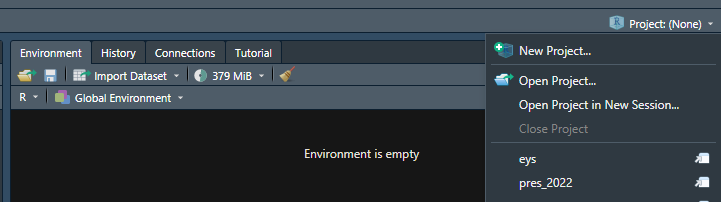
\includegraphics[width=0.6\linewidth]{./figs/1} \end{center}

\begin{itemize}
\tightlist
\item
  Si les aparece este mensaje, en lo posible intenten no guardar. La
  gracia es que todo esté guardado en código. De todas formas, fíjense
  bien en que no pierdan información. Si no, guarden por si acaso.
\end{itemize}

\begin{Shaded}
\begin{Highlighting}[]
\NormalTok{knitr}\SpecialCharTok{::}\FunctionTok{include\_graphics}\NormalTok{(}\StringTok{"./figs/2.PNG"}\NormalTok{)}
\end{Highlighting}
\end{Shaded}

\begin{center}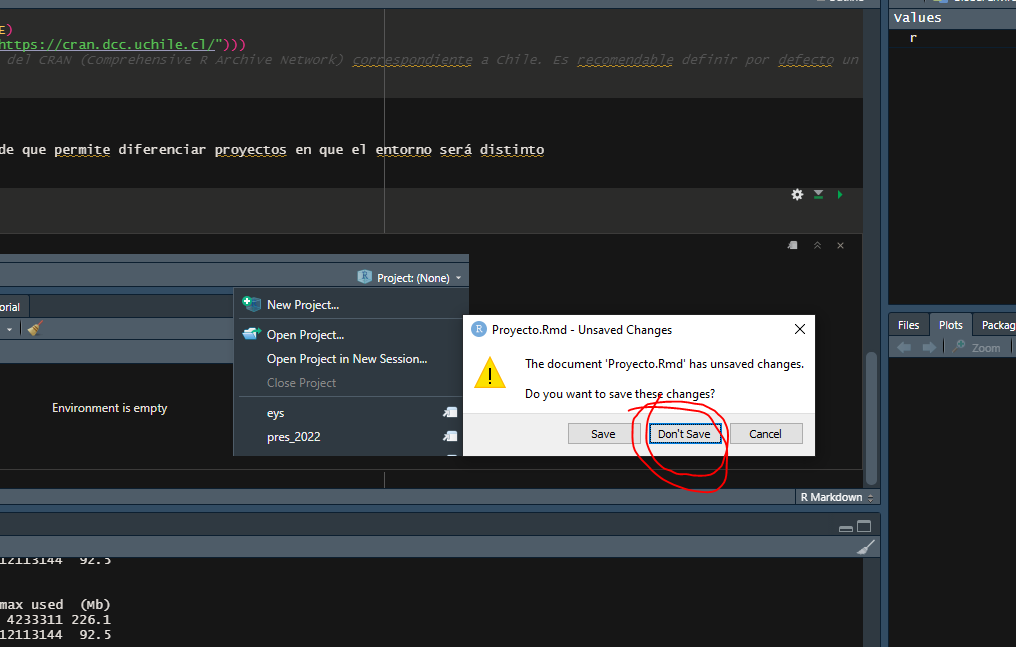
\includegraphics[width=0.6\linewidth]{./figs/2} \end{center}

\begin{itemize}
\tightlist
\item
  Van aquí y ponen ``New Directory (Nuevo directorio/carpeta)'', si es
  que quieren empezar el proyecto en una nueva carpeta, o ``Existing
  Directory (Directorio existente)'', si es que quieren hacerlo en una
  carpeta que ya tienen. En este ejemplo lo hacemos en un New Directory.
  Este directorio será el mismo cuando utilicemos \texttt{getwd()}. Esto
  además hace no necesario utilizar \texttt{setwd()}
\end{itemize}

\begin{Shaded}
\begin{Highlighting}[]
\NormalTok{knitr}\SpecialCharTok{::}\FunctionTok{include\_graphics}\NormalTok{(}\StringTok{"./figs/3.PNG"}\NormalTok{)}
\end{Highlighting}
\end{Shaded}

\begin{center}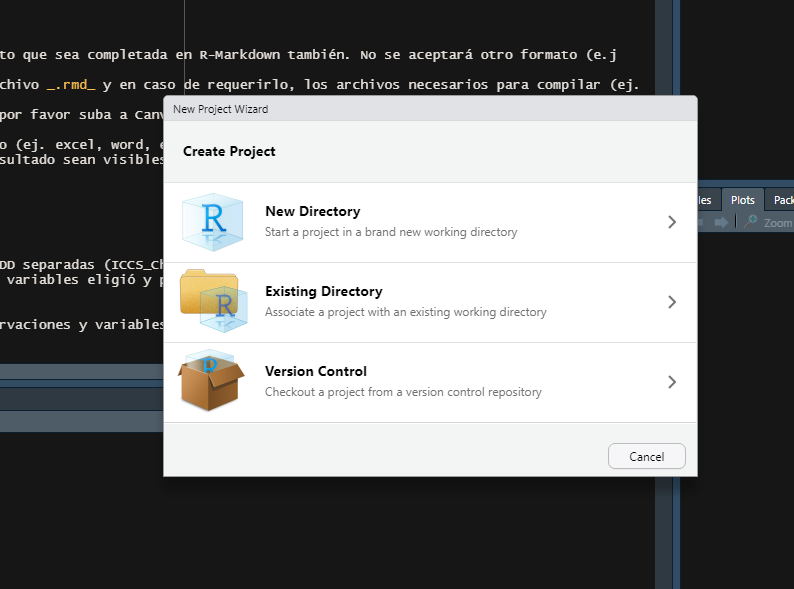
\includegraphics[width=0.6\linewidth]{./figs/3} \end{center}

\begin{itemize}
\tightlist
\item
  Ahí defino el nombre de la carpeta, dentro de qué carpeta estará, y si
  la abriré en otra sesión (en otra ventana de Rstudio).
\end{itemize}

\begin{Shaded}
\begin{Highlighting}[]
\NormalTok{knitr}\SpecialCharTok{::}\FunctionTok{include\_graphics}\NormalTok{(}\StringTok{"./figs/4.PNG"}\NormalTok{)}
\end{Highlighting}
\end{Shaded}

\begin{center}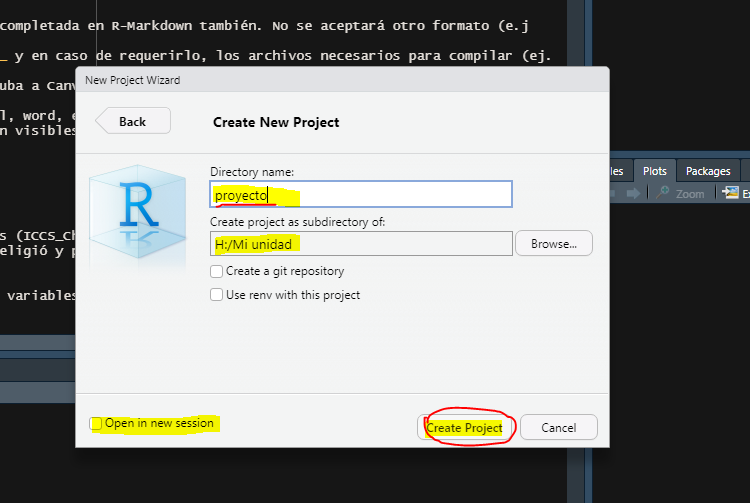
\includegraphics[width=0.6\linewidth]{./figs/4} \end{center}

\begin{itemize}
\tightlist
\item
  Se abre la nueva ventana. Aquí todavía no tenemos ningún archivo en la
  carpeta del directorio. Si no se ve de esta forma puede dar click a
  \texttt{Cntrl+\ Alt+\ Shift+\ 0} en Windows, y
  \texttt{Cmd+\ Alt+\ Shift+\ 0} en Mac, para ver los cuatro principales
  módulos de R.
\end{itemize}

\hypertarget{paso-2.-abriendo-cuxf3digo}{%
\subsection{Paso 2. Abriendo código}\label{paso-2.-abriendo-cuxf3digo}}

\begin{Shaded}
\begin{Highlighting}[]
\NormalTok{knitr}\SpecialCharTok{::}\FunctionTok{include\_graphics}\NormalTok{(}\StringTok{"./figs/5.PNG"}\NormalTok{)}
\end{Highlighting}
\end{Shaded}

\begin{center}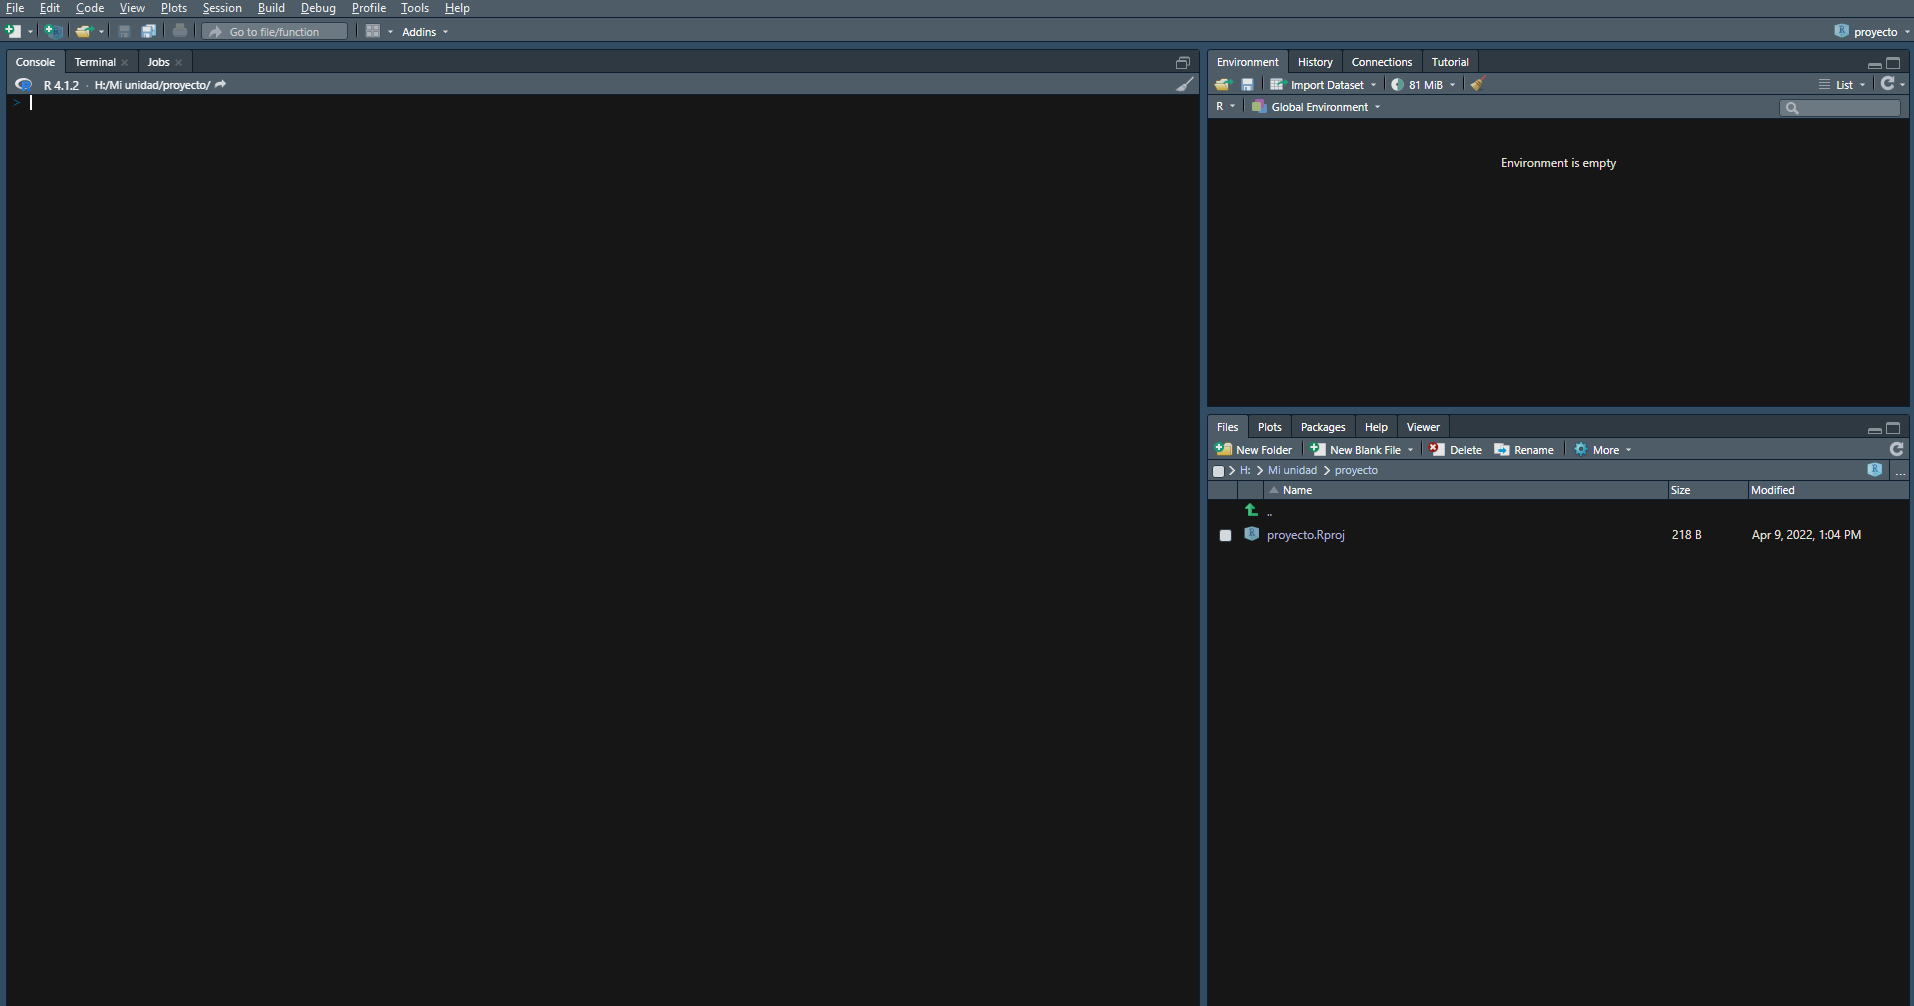
\includegraphics[width=0.6\linewidth]{./figs/5} \end{center}

\begin{itemize}
\tightlist
\item
  Puede abrir un archivo ya sea generando una libreta de texto abierto,
  o bien cargar otro archivo un .RMD (en este ejemplo. )
\end{itemize}

\begin{Shaded}
\begin{Highlighting}[]
\NormalTok{knitr}\SpecialCharTok{::}\FunctionTok{include\_graphics}\NormalTok{(}\StringTok{"./figs/6.PNG"}\NormalTok{)}
\end{Highlighting}
\end{Shaded}

\begin{center}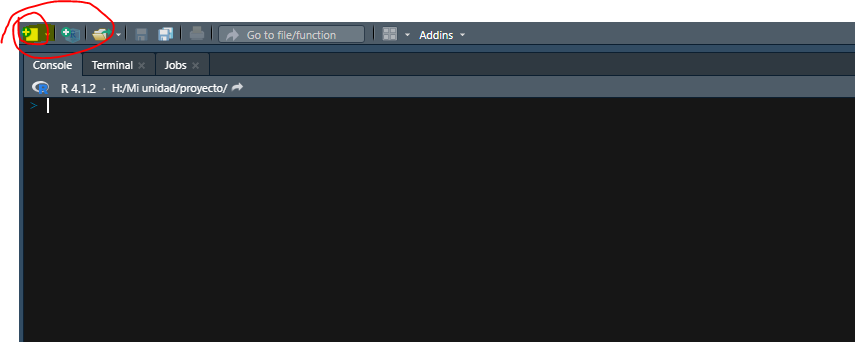
\includegraphics[width=0.6\linewidth]{./figs/6} \end{center}

\begin{itemize}
\tightlist
\item
  Vamos a abrir un archivo.
\end{itemize}

\begin{Shaded}
\begin{Highlighting}[]
\NormalTok{knitr}\SpecialCharTok{::}\FunctionTok{include\_graphics}\NormalTok{(}\StringTok{"./figs/7.PNG"}\NormalTok{)}
\end{Highlighting}
\end{Shaded}

\begin{center}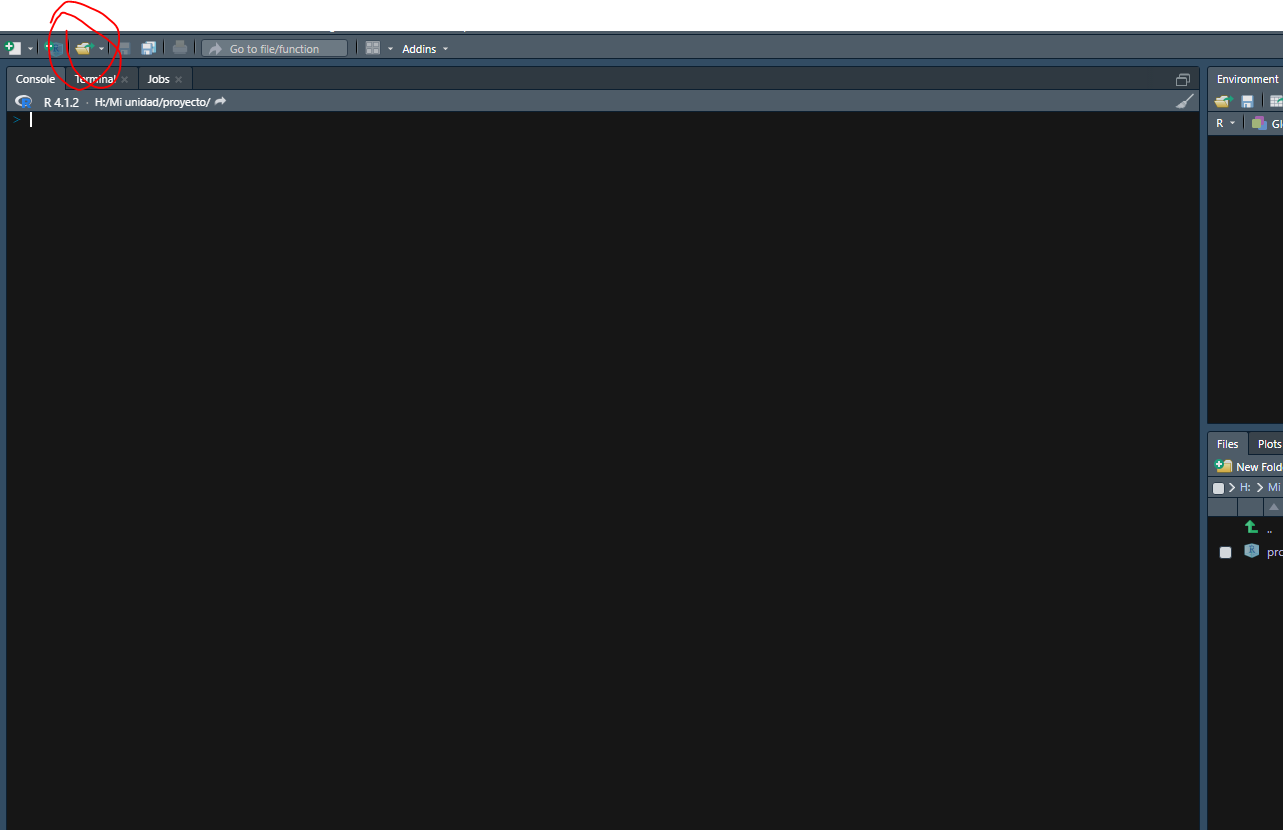
\includegraphics[width=0.6\linewidth]{./figs/7} \end{center}

\begin{itemize}
\tightlist
\item
  Antes decidí incorporar a la carpeta el Rmarkdown (.RMD) en la carpeta
  de mi proyecto como buena práctica.
\end{itemize}

\begin{Shaded}
\begin{Highlighting}[]
\NormalTok{knitr}\SpecialCharTok{::}\FunctionTok{include\_graphics}\NormalTok{(}\StringTok{"./figs/8.PNG"}\NormalTok{)}
\end{Highlighting}
\end{Shaded}

\begin{center}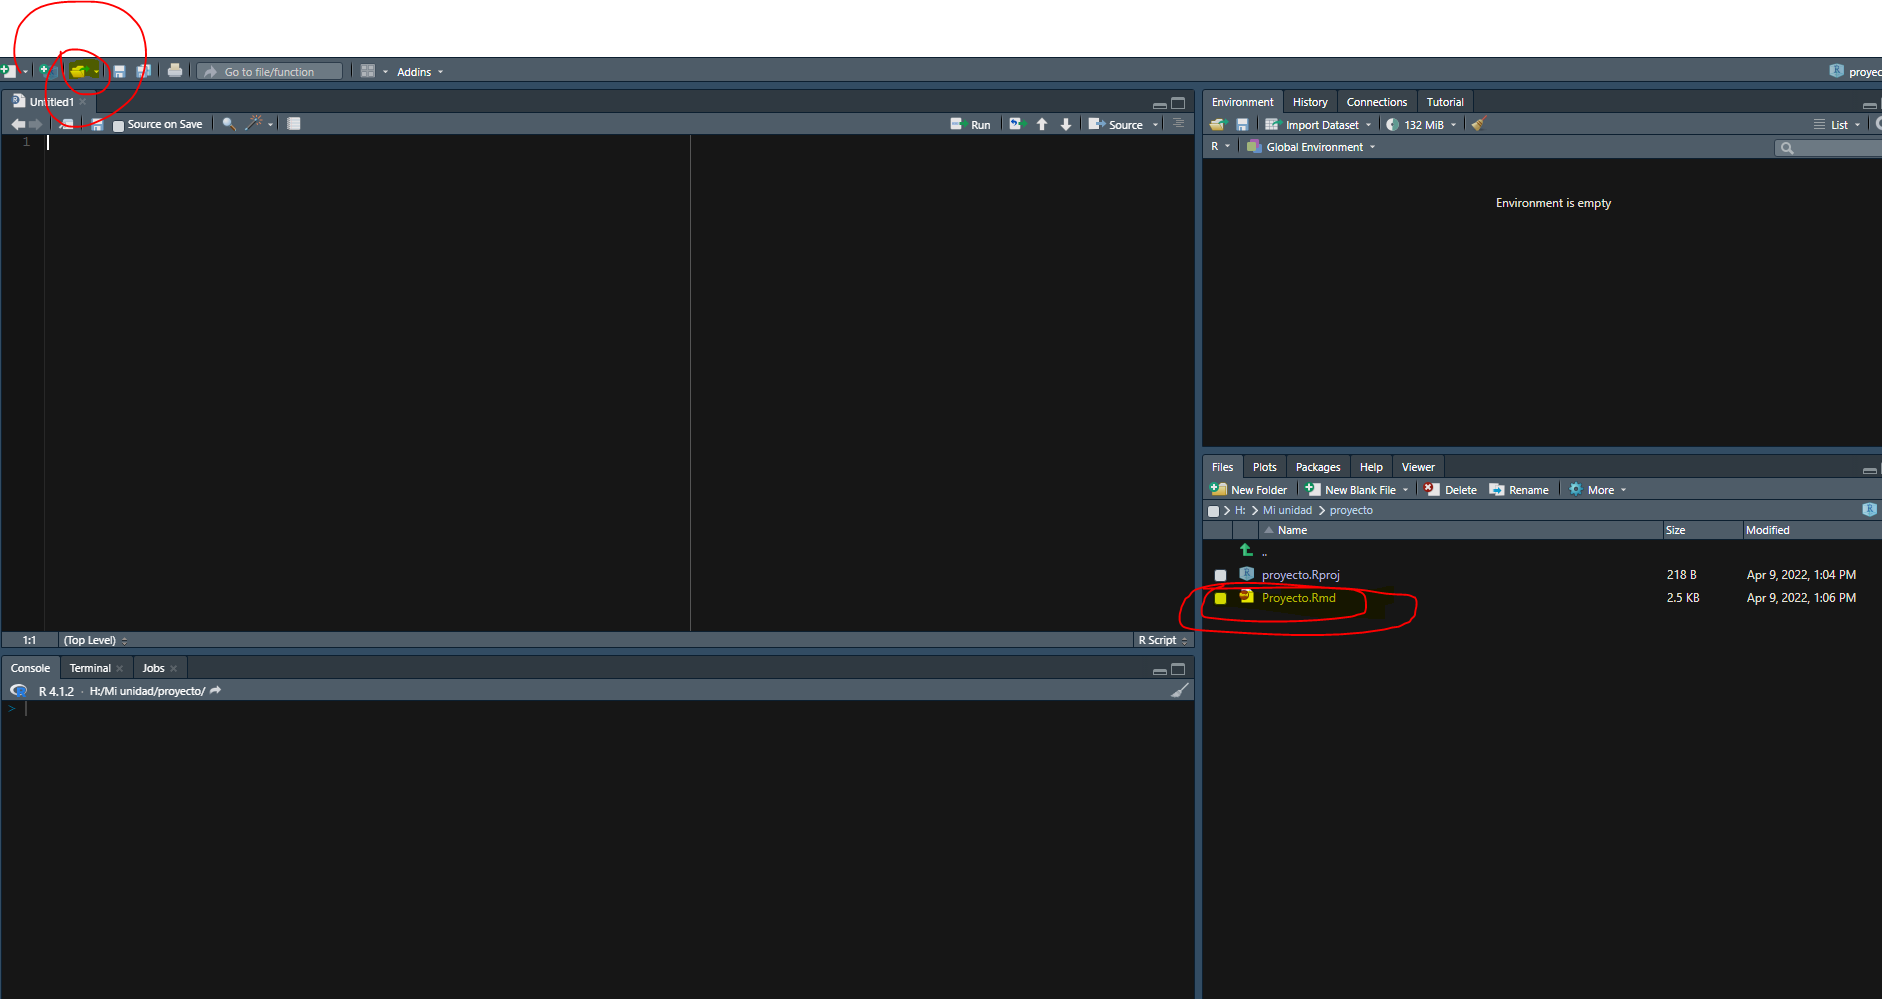
\includegraphics[width=0.6\linewidth]{./figs/8} \end{center}

\begin{itemize}
\tightlist
\item
  Abro el .RMD
\end{itemize}

\begin{Shaded}
\begin{Highlighting}[]
\NormalTok{knitr}\SpecialCharTok{::}\FunctionTok{include\_graphics}\NormalTok{(}\StringTok{"./figs/9.PNG"}\NormalTok{)}
\end{Highlighting}
\end{Shaded}

\begin{center}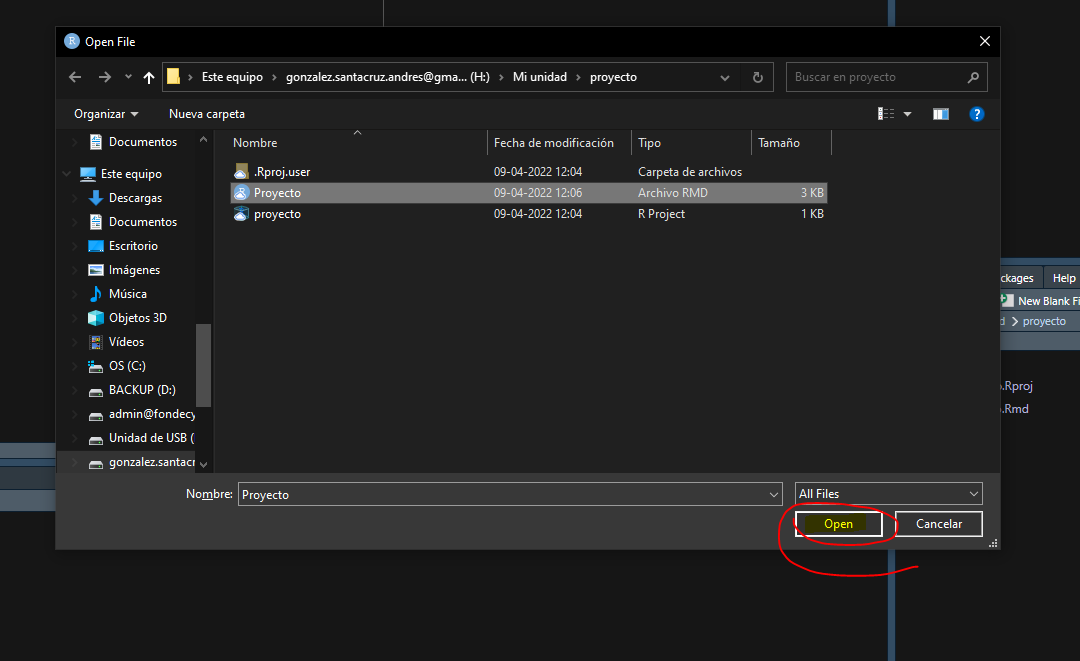
\includegraphics[width=0.6\linewidth]{./figs/9} \end{center}

\begin{itemize}
\tightlist
\item
  Ahora, dado que en este proyecto estoy trabajando con figuras
  (capturas de pantalla), las incorporaré también a este carpeta aunque
  las dejaré en una subcarpeta llamada ``figs'', cosa que sea fácil
  llamarlas con un \texttt{knitr::include\_graphics("./figs/9.PNG")},
  por ejemplo.
\end{itemize}

\begin{Shaded}
\begin{Highlighting}[]
\NormalTok{knitr}\SpecialCharTok{::}\FunctionTok{include\_graphics}\NormalTok{(}\StringTok{"./figs/10.PNG"}\NormalTok{)}
\end{Highlighting}
\end{Shaded}

\begin{center}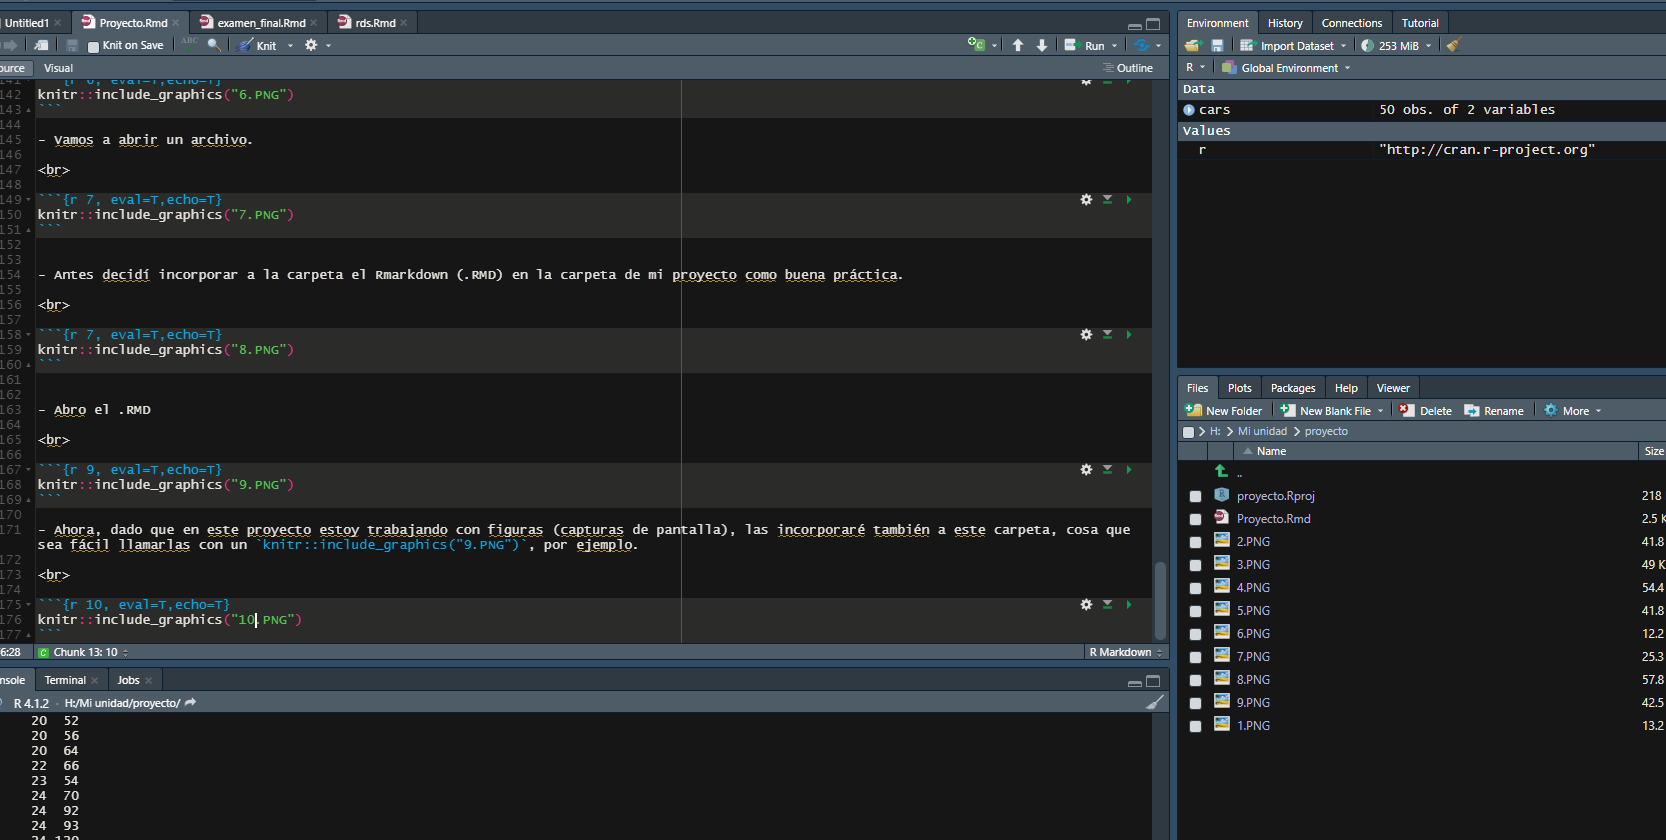
\includegraphics[width=0.6\linewidth]{./figs/10} \end{center}

\begin{itemize}
\tightlist
\item
  Nos fijamos que nuestro avance quede guardado en nuestro
  \emph{RMarkdown}, siempre que podamos. Ya sea con el disco duro
  redondeado o presionando \texttt{Cntrl+S}.
\end{itemize}

\begin{Shaded}
\begin{Highlighting}[]
\NormalTok{knitr}\SpecialCharTok{::}\FunctionTok{include\_graphics}\NormalTok{(}\StringTok{"./figs/11.PNG"}\NormalTok{)}
\end{Highlighting}
\end{Shaded}

\begin{center}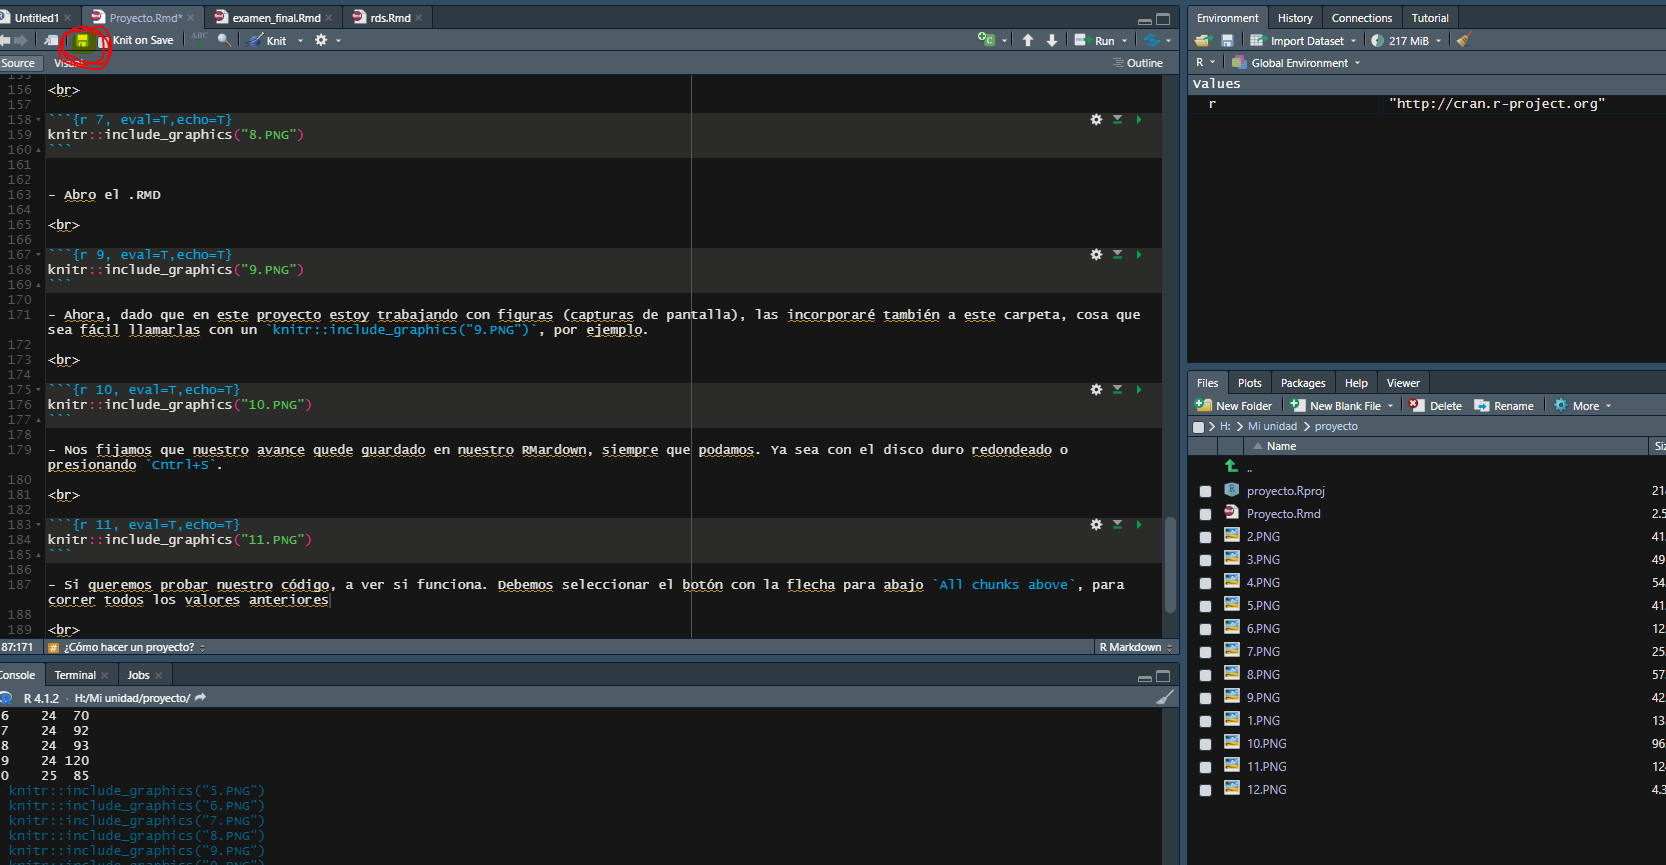
\includegraphics[width=0.6\linewidth]{./figs/11} \end{center}

\hypertarget{paso-3.-probar-el-cuxf3digo}{%
\subsection{Paso 3. Probar el
código}\label{paso-3.-probar-el-cuxf3digo}}

\begin{itemize}
\tightlist
\item
  Si queremos probar nuestro código, a ver si funciona. Debemos
  seleccionar el botón con la flecha para abajo
  \texttt{All\ chunks\ above}, para correr todos los chunks anteriores,
  o bien la flecha verde a la derecha para sólo desplegar
  (\texttt{Run\ current\ chunk}).
\end{itemize}

\begin{Shaded}
\begin{Highlighting}[]
\NormalTok{knitr}\SpecialCharTok{::}\FunctionTok{include\_graphics}\NormalTok{(}\StringTok{"./figs/12.PNG"}\NormalTok{)}
\end{Highlighting}
\end{Shaded}

\begin{center}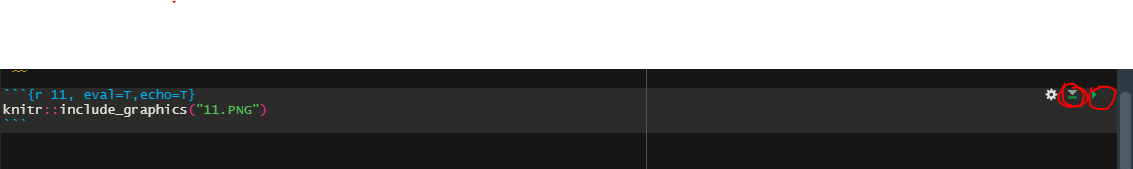
\includegraphics[width=0.6\linewidth]{./figs/12} \end{center}

\begin{itemize}
\tightlist
\item
  Vemos si hay errores en los chunks. Si no los hay, podemos generar un
  chunk nuevo cargando las variables. En este caso instalo
  \texttt{pacman}, y cargo \texttt{knitr} y \texttt{dplyr}. Luego cargo
  la base de datos \texttt{mtcars} del paquete dplyr.
\end{itemize}

\begin{Shaded}
\begin{Highlighting}[]
\ControlFlowTok{if}\NormalTok{(}\SpecialCharTok{!}\FunctionTok{require}\NormalTok{(pacman))\{}\FunctionTok{install.packages}\NormalTok{(}\StringTok{"pacman"}\NormalTok{)\}}
\CommentTok{\#INSTALO PAQUETES}
\NormalTok{pacman}\SpecialCharTok{::}\FunctionTok{p\_load}\NormalTok{(knitr, dplyr)}
\CommentTok{\#Traigo la base mtcars}
\FunctionTok{data}\NormalTok{(mtcars)}
\end{Highlighting}
\end{Shaded}

\begin{Shaded}
\begin{Highlighting}[]
\NormalTok{knitr}\SpecialCharTok{::}\FunctionTok{include\_graphics}\NormalTok{(}\StringTok{"./figs/13.PNG"}\NormalTok{)}
\end{Highlighting}
\end{Shaded}

\begin{center}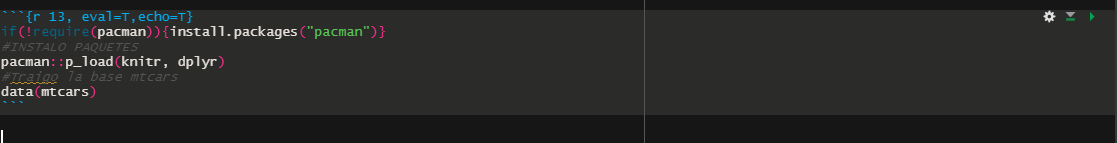
\includegraphics[width=0.6\linewidth]{./figs/13} \end{center}

\begin{itemize}
\tightlist
\item
  Ahora tendré la base de datos como promesa (\texttt{promise}) arriba.
  Si le doy a escribir la estructura usando en la consola
  \texttt{str(mtcars)}, me aparecerá en mi entorno.
\end{itemize}

\begin{Shaded}
\begin{Highlighting}[]
\NormalTok{knitr}\SpecialCharTok{::}\FunctionTok{include\_graphics}\NormalTok{(}\StringTok{"./figs/14a.PNG"}\NormalTok{)}
\end{Highlighting}
\end{Shaded}

\begin{center}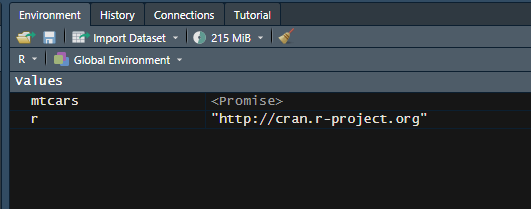
\includegraphics[width=0.6\linewidth]{./figs/14a} \end{center}

\begin{Shaded}
\begin{Highlighting}[]
\NormalTok{knitr}\SpecialCharTok{::}\FunctionTok{include\_graphics}\NormalTok{(}\StringTok{"./figs/14b.PNG"}\NormalTok{)}
\end{Highlighting}
\end{Shaded}

\begin{center}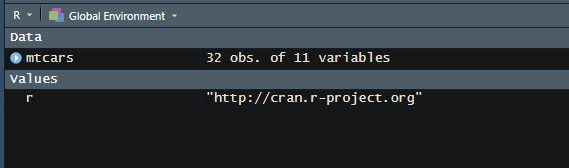
\includegraphics[width=0.6\linewidth]{./figs/14b} \end{center}

\begin{itemize}
\tightlist
\item
  Una vez que tengo mi base de datos lista, además de guardar mi
  Rmarkdown (Cntrl+ S), puedo guardar mis datos de R para cargarlos a
  futuro. Recuerde que el formato de los datos guardados será
  \texttt{*.RData}.
\end{itemize}

\begin{Shaded}
\begin{Highlighting}[]
\NormalTok{knitr}\SpecialCharTok{::}\FunctionTok{include\_graphics}\NormalTok{(}\StringTok{"./figs/15.PNG"}\NormalTok{)}
\end{Highlighting}
\end{Shaded}

\begin{center}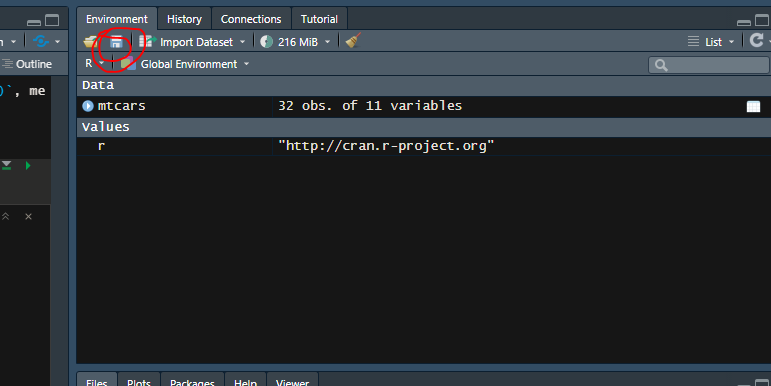
\includegraphics[width=0.6\linewidth]{./figs/15} \end{center}

\begin{itemize}
\tightlist
\item
  Una vez que tengo mi base de datos lista, además de guardar mi
  Rmarkdown (Cntrl+ S), puedo guardar mis datos de R para cargarlos a
  futuro. Recuerde que el formato de los datos guardados será
  \texttt{*.RData}.
\end{itemize}

\hypertarget{paso-4.-cerrar-proyecto}{%
\subsection{Paso 4. Cerrar proyecto}\label{paso-4.-cerrar-proyecto}}

\begin{Shaded}
\begin{Highlighting}[]
\NormalTok{knitr}\SpecialCharTok{::}\FunctionTok{include\_graphics}\NormalTok{(}\StringTok{"./figs/16.PNG"}\NormalTok{)}
\end{Highlighting}
\end{Shaded}

\begin{center}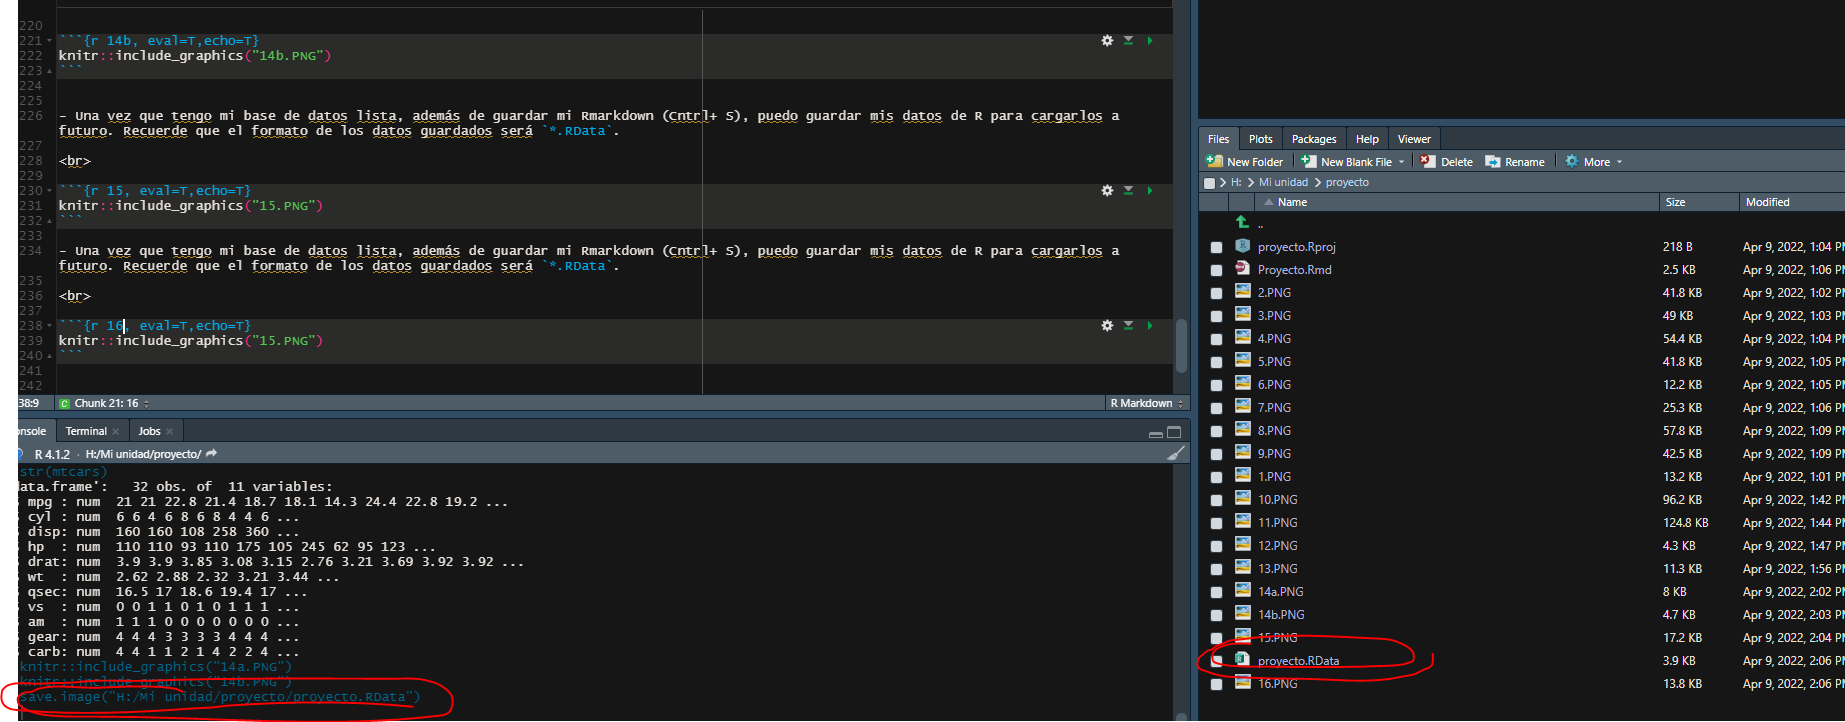
\includegraphics[width=0.6\linewidth]{./figs/16} \end{center}

\begin{itemize}
\tightlist
\item
  Ahora que guardamos todo, podemos cerrar el proyecto (cerrar R). Si se
  fijan, nos abrirá automáticamente el último proyecto abierto (en
  nuestro caso, este). Debemos \textbf{siempre generar un proyecto
  nuevo, ojalá en otra carpeta, siempre que trabajemos en una tarea
  distinta}. Por lo mismo, debemos siempre seguir los pasos aquí, y
  partir nuestro proyecto limpiando el entorno, y limpiando el espacio
  virtual (la RAM) \texttt{rm(list=ls());gc()}.
\end{itemize}

\end{document}
